\section{Mediciones de validación de proyecto de ejemplo: Phaser}

\subsection{Prueba diseñada:}

Los pasos propuestos para validar el correcto funcionamiento del efecto phaser en la LCDK son los que se presentan a continuación:

\begin{enumerate}
    \item Con la placa LCDK programada en modo bypass, usar de señal de entrada al codec de audio una señal de ruido blanco (y por lo tanto de espectro distribuido) de 1 Vpp obtenido a partir de un generador de señales.
    
    Este es importante por 2 razones:
    \begin{itemize}
        \item Verificar el funcionamiento del modo bypass.
        \item Contar con señal de referencia para futuras comparaciones.%La señal de ruido blanco es de espectro distribuido, por lo que en el espectro del ruido filtrado se podrá apreciar la respuesta en frecuencia del filtro que se está usando en un momento en particular.
    \end{itemize}
    
    Se utiliza una señal de 1 Vpp para no dañar el codec.
    
    \item Importar archivo de audio en MATLAB y obtener su espectrograma con el script \texttt{Spectrogram\_test}, previamente implementado.
    
    El espectrograma permitirá verificar que la señal sea de espectro distribuido en el tiempo
    
    \item Repetir paso 1 con phaser activado.
    
    El espectro de está señal se verá afectado por el filtro dinámico.
    
    \item Importar archivo de audio grabado en paso anterior en MATLAB y obtener su espectrograma con el script del paso 2.
    
    En el espectrograma se apreciarpa el movimiento de los nulos el filtro notch en el tiempo, por lo que el funcionamiento del phaser quedará validado.
    
\end{enumerate}
\subsection{Resultados de Validación:}
Para esta parte se utilizó el código \texttt{Spectrogram\_test}.

El espectrograma de la señal de ruido blanco pasada por la LCDK en modo bypass se muestra en a figura \ref{fig:bypass}. Se aprecia el espectro plano esperado, salvo por otro lado se observa una caída en el espectro en torno a los 8 kHz. Esta caída se debe a que el códec de audio posee un filtro pasabajos a la frecuencia de Nyquist ($\tfrac{16}{2}$ kHz) con el fin de evitar los efectos de doblaje en frecuencia.  
\begin{figure}[H]
    \centering
    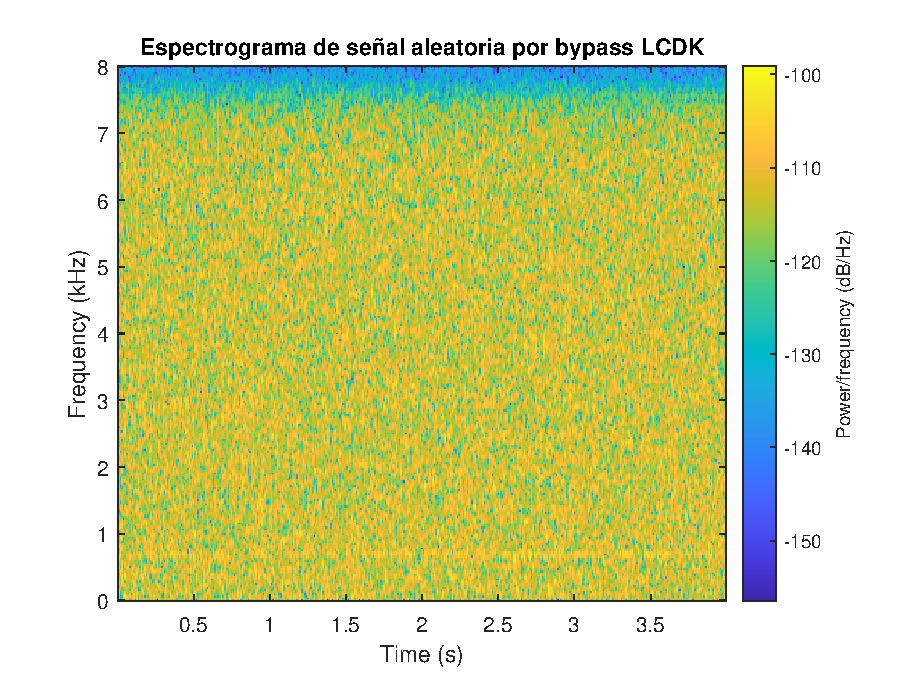
\includegraphics[width = .8\linewidth]{figures/bypass_spectrogram.eps}
    \caption{Espectrograma de señal de ruido blanco pasada por la LCDK programada en modo bypass. Ventanas 20 ms sin overlap.}
    \label{fig:bypass}
\end{figure}

El espectrograma de la señal de ruido blanco pasada por la LCDK en modo phaser se muestra en a figura \ref{fig:bypass}. Se aprecia el cambio de la frecuecias atenuadas por el filtro notch en el tiempo, por lo que se valida el correcto funcionamiento del efecto de audio.

\begin{figure}[H]
    \centering
    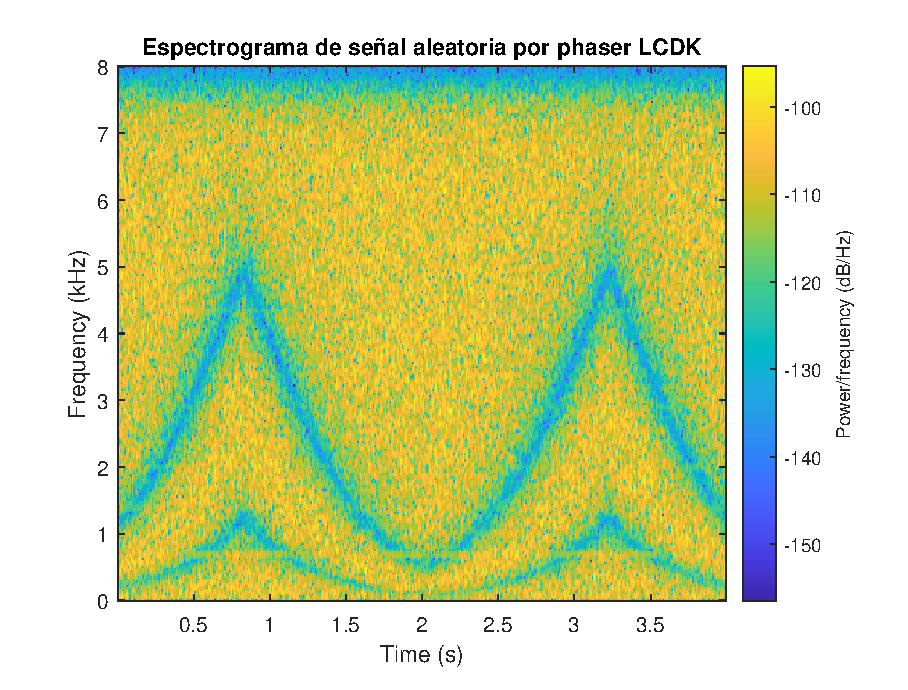
\includegraphics[width = .8\linewidth]{figures/phaser_spectrogram.eps}
    \caption{Espectrograma de señal de ruido blanco pasada por la LCDK programada en modo phaser. Ventanas 20 ms sin overlap.}
    \label{fig:phaser}
\end{figure}


